A 1823 Theorem by Sturm states that given a triangle, the area of the {\em pedal triangle} with respect to a point $M$ is constant for all $M$ on a circle centered on the circumcenter $X_3$ \cite[Thm. 7.28, page 221]{ostermann2012}, Figure~\ref{fig:sturm}.

\begin{figure}
    \centering
    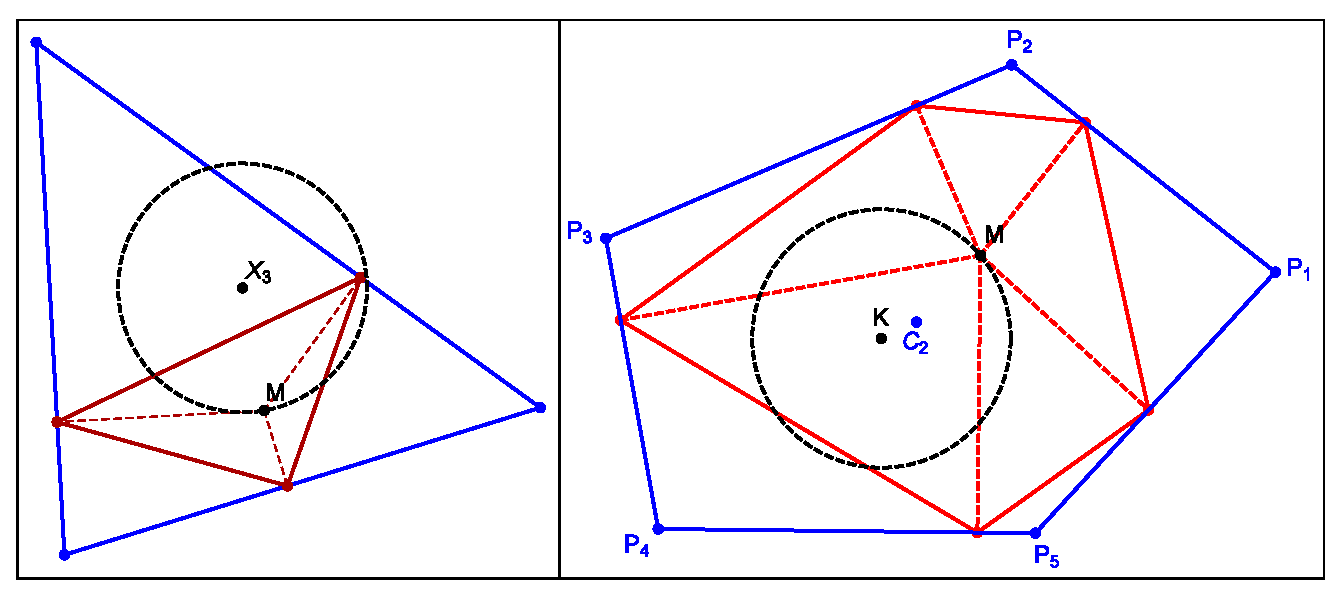
\includegraphics[width=\textwidth]{pics/0006_sturm_and_steiner.eps}
    \caption{\textbf{Left}: Sturm's Theorem (1823) states that the area of the pedal triangle (red) of a reference triangle (blue) is invariant for all points $M$ lying a circles (dashed black) centered on the circumcenter $X_3$. \textbf{Right}: in 1825, Steiner generalizes this to polygons: the area of the pedal polygon (red) to an N-gon (blue) is constant for all $M$ over a circle centered on $K$, the curvature centroid. $C_2$ denotes the polygon's center of area.}
    \label{fig:sturm}
\end{figure}

In 1825 Steiner generalized it as follows: given a polygon with vertices $P_i,i=1,{\ldots}N$, the area of its pedal polygon with respect to $M$ is invariant for $M$ on a circle centered on Steiner's {\em curvature centroid} $K$, given by \cite{steiner1838}:

\begin{equation*}
    K = \frac{\sum_i{\sin(2\theta_i) P_i}}{\sum_i{\sin(2\theta_i)}}
%    \label{eq:centroid-steiner}
\end{equation*}

\noindent where $\theta_i$ are the internal angles, $i=1,\cdots,N$. In the same publication Steiner also proves that the pedal polygon with respect to $K$ has extremal area. Note for $N=3$, $K=X_3$ as the latter has barycentrics of $\sin(2\theta_i)$ \cite{etc}. This is consistent with the fact that pedal polygons with respect to points on the circumcircle have constant area (in fact they have zero area, their vertices lie on the Simson line \cite[Simson Line]{mw}).

Steiner further generalized the above to the case of a closed plane curve $\mathcal{C}$, by approximating it with a polygon where $N{\rightarrow}\infty$. Let the {\em pedal curve} $\mathcal{C}_p$ of $\mathcal{C}$ with respect to a point $M$ be the locus of the foot of the perpendicular dropped from $M$ onto 
  the tangent at a point $P(t)$ to $\mathcal{C}$
  for all $t$; see Figure~\ref{fig:steiner-general}. With $N{\rightarrow}\infty$,
provided that the total curvature of $\mathcal{C}$ is non-zero (i.e., non-zero winding number), $K$ becomes \cite{steiner1838}:

\begin{equation}
    K = \frac{\int{\kappa(s) P(s).ds}}{\int{\kappa(s).ds}}
    \label{eqn:steiner-k}
\end{equation}

\noindent where $\kappa(s)$ is the curvature and $s$ is arc length. Referring to Figure~\ref{fig:steiner-general}, we recall a result by Jakob Steiner \cite{steiner1838}:  

\begin{theorem*}[Steiner, 1825]
The area of the pedal curve is constant for  points $M$ lying on circles centered on $K$.
%\label{thm:pedal}
\end{theorem*}

\begin{figure}
    \centering
    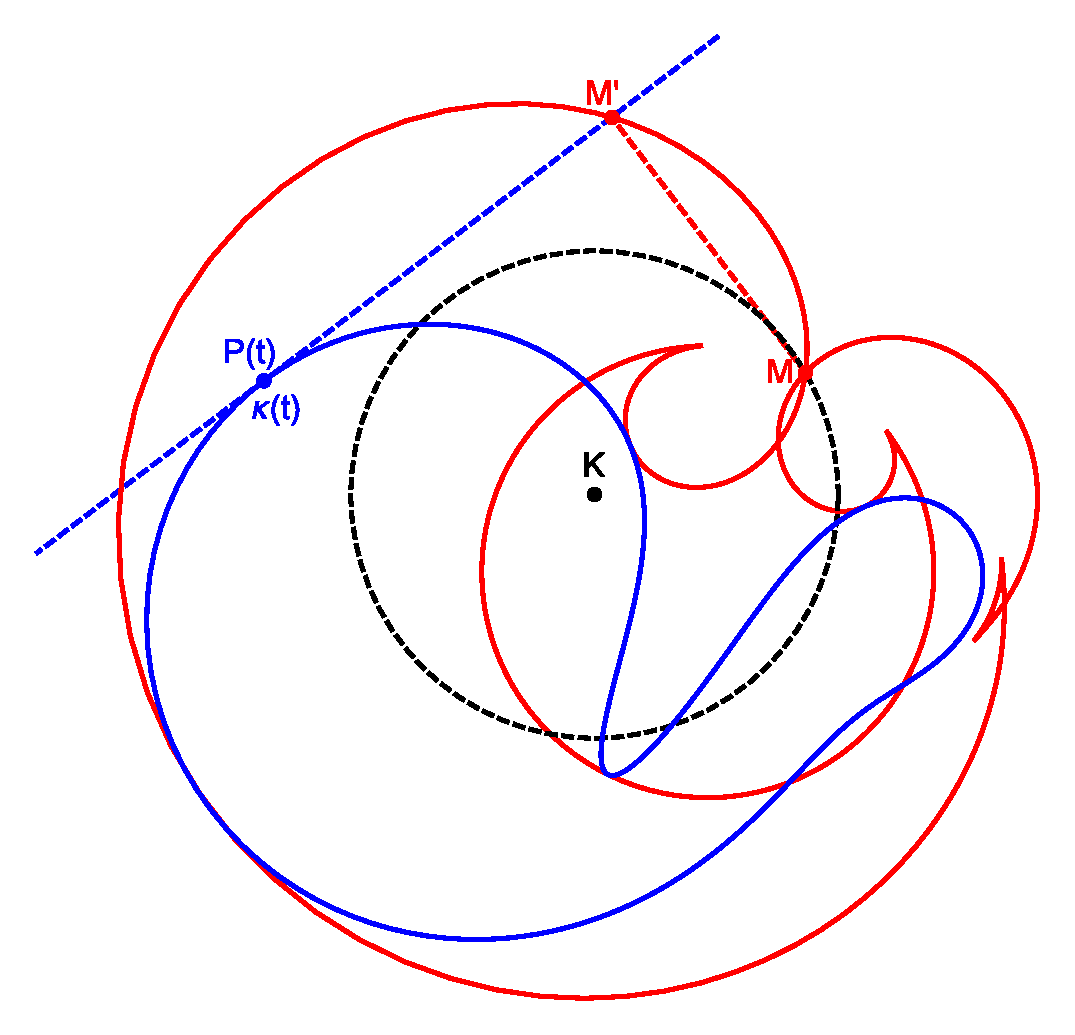
\includegraphics[width=.5\textwidth]{pics/0007_general_poly_steiner.eps}
    \caption{A generic closed curve $\mathcal{C}$ (blue) and its pedal curve (red), defined as the locus of the foot $M'$ of perpendiculars dropped from $M$
    onto the tangent to $\mathcal C$ at $P(t)$.
     The Steiner curvature centroid $K$ is obtained by averaging the curvature $\kappa(t)$ over all $P(t)$; see equation~\eqref{eqn:steiner-k}. The signed area of the pedal polygon is constant for $M$ lying in a circle centered on $K$.}
    \label{fig:steiner-general}
\end{figure}

From symmetry:

\begin{lemma}
For the ellipse and its evolute (an astroid), $K=O$.
%\label{lem:ellipse-k}
\end{lemma}

%Note: when expressed in line %coordinates, the cusps of the evolute %are regular. Specifically, cusps of the %evolute are inflection points of its %dual \cite{fischer2001,akopyan2007-conic%s}. 

Referring to Figure~\ref{fig:pedal-contrapedal}:

\begin{figure}
    \centering
    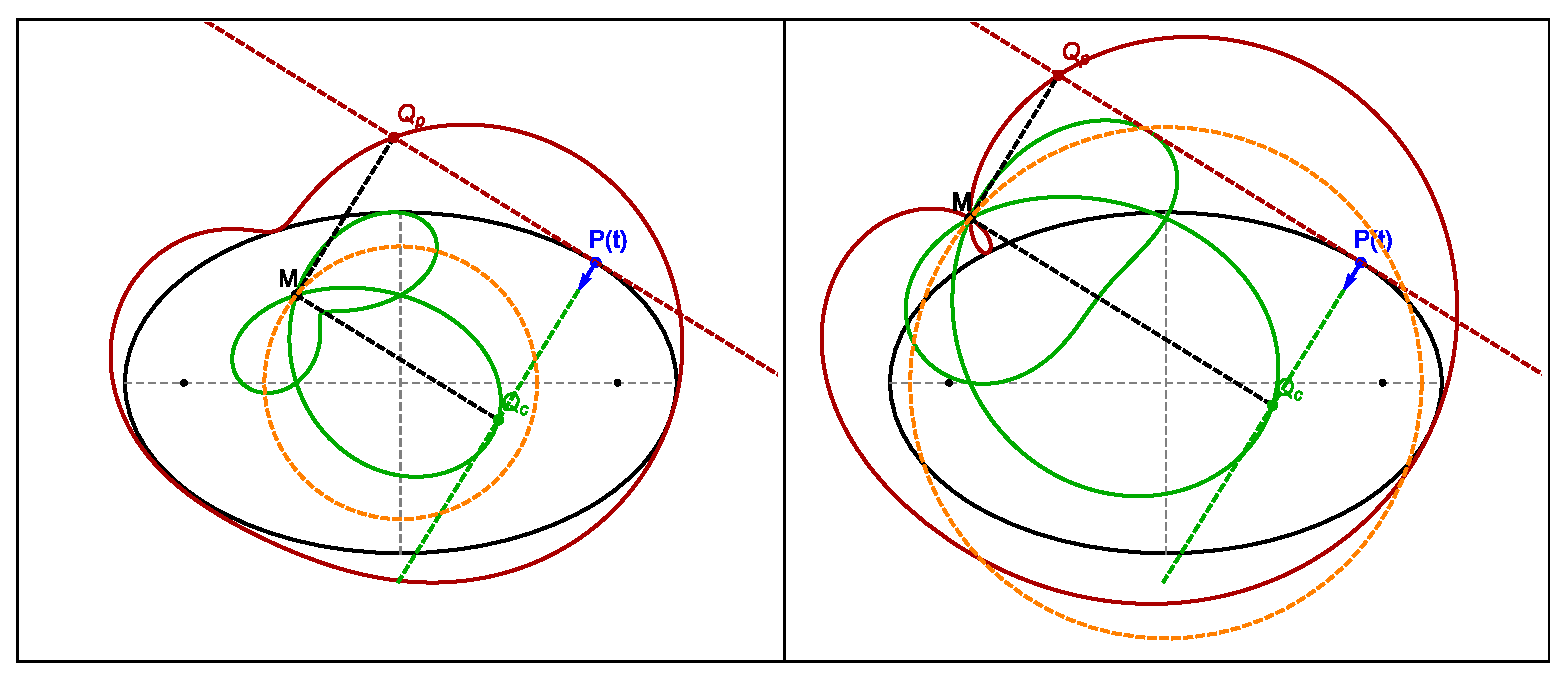
\includegraphics[width=\textwidth]{pics/0020_iso_areas.eps}
    \caption{\textbf{Left:} The areas $A_p$ (resp. $A_c$) of the Pedal Curve $\mathcal{E}_{p}$ (red) (resp. Contrapedal Curve $\mathcal{E}_{c}$, green) are invariant for all $M$ on a circle (orange) concentric with the ellipse. \textbf{Right:} An iso-area concentric circle (orange) of radius larger than the minor axis of the ellipse.}
    \label{fig:pedal-contrapedal}
\end{figure}

\begin{corollary}
The area $A_p$ of the pedal curve is invariant for $M$ on a circle concentric with $\mathcal{E}$.
\end{corollary}

As illustrated for an ellipse in Figure~\ref{fig:contrapedal}, in general, the contrapedal curve is the pedal curve with respect to the evolute \cite[Contrapedal Curve]{mw} and:

\begin{corollary}
The area $A_c$ of the contrapedal curve is invariant for $M$ on a circle concentric with $\mathcal{E}$.
\end{corollary}

Let the term $\theta$-evolutoid denote the envelope of $\theta$-rotated tangents to a curve; see Figure~\ref{fig:evolutoid}.

\begin{figure}
    \centering
    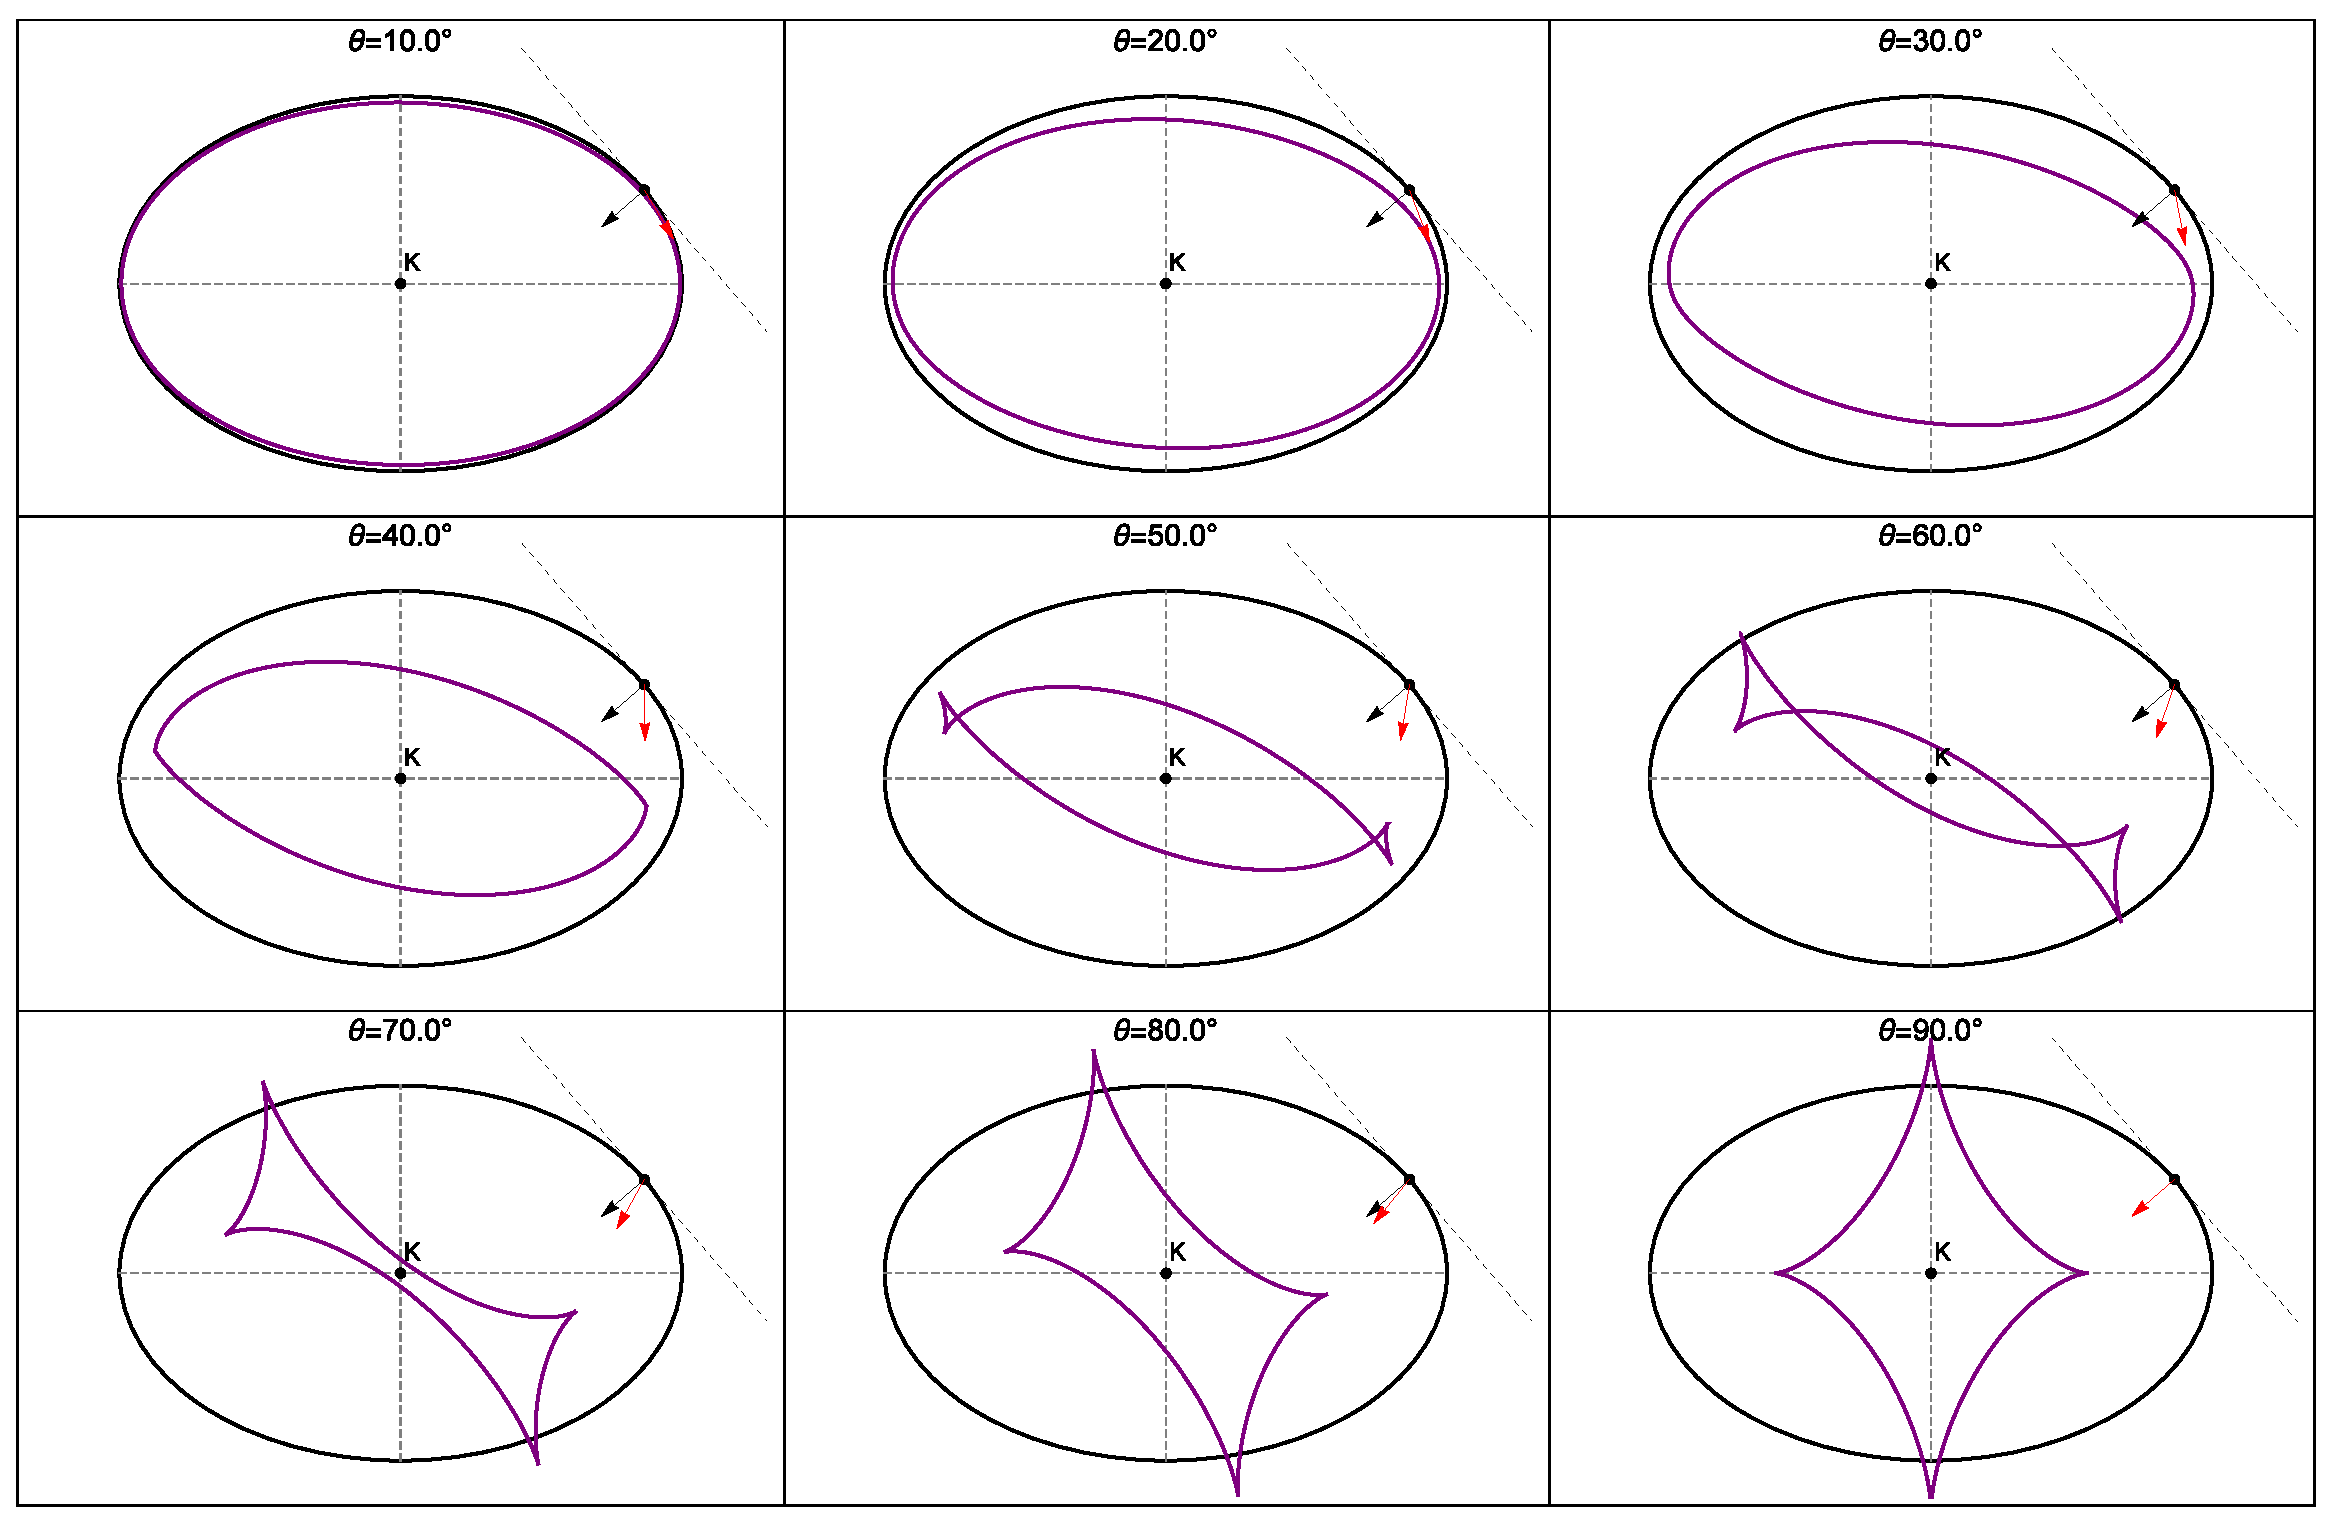
\includegraphics[width=\textwidth]{pics/0015_evolutoids.eps}
    \caption{The $\theta$-evolutoid \cite{jesus2015,jesus2014} (purple, envelope of tangents rotated by $\theta$) for an $a/b=1.5$ ellipse, $\theta=10,\ldots,90$ degrees. The bottom-right figure ($\theta=90^\circ$) is the ellipse evolute. Also shown are the normal (black arrow) and rotated tangent (red arrow) for a point in the 1st quadrant. Since these curves are centrally symmetric, the Steiner curvature centroid $K$ lies at the ellipse center.}
    \label{fig:evolutoid}
\end{figure}

\begin{lemma}
The $\theta$-evolutoid to an ellipse has $K=O$, for any $\theta$.  
\label{lem:evolutoid-k}
\end{lemma}

This stems from the fact that for all $\theta$, the $\theta$-evolutoid remains symmetric with respect to the origin $O$.

\begin{corollary}
The area $A_{\theta}$ of the rotated contrapedal curve is invariant for $M$ on a circle concentric with $\mathcal{E}$.
\end{corollary}

This stems from the fact that the rotated pedal curve $\mathcal{E}_{\theta}$ is the pedal with respect to a $\theta$-evolutoid and Lemma~\ref{lem:evolutoid-k}.

\begin{theorem}
The area $A_\mu$ of the interpolated pedal curve is invariant for $M$ on a circle concentric with $\mathcal{E}$.
\end{theorem}

\begin{proof}
Proposition~\ref{prop:amu-concave} in Section~\ref{sec:epilogue} shows that for any closed curve with non-zero total curvature (the denominator of Equation~\eqref{eqn:steiner-k}),  $A_{\mu}$ is a fixed linear function of $A_p$ and $A_c$. Since both $A_p$ and $A_c$ are constant for $M$ on circles centered on $K=O$, the result follows.
\end{proof}
